\section{Related Work}
\label{sec:related}

%===================================================
\noindent
\textbf{Urban Traffic Visual Analytics}.
In order to facilitate exploration of human/vehicle/goods movement in cities, many visual analytics for urban traffic data have been developed.
These visual analytics can facilitate understanding of urban dynamics and human activities, and also enhance traffic management and assessment.
Systematic reviews of these works are presented in~\cite{chen_survey_2015, andrienko2017visual}.
In particular, some visual analytics have been specifically developed for studying OD trails in urban traffic.
Among them, advanced indexing methods (e.g.,~\cite{ferreira2013visual, zeng_2015_visualizing}) and new interaction models (e.g.,~\cite{kruger_trajectorylenses_2013, zeng_2015_visualizing}), have been developed to facilitate movement query.
After filtering OD trails, these visual analytics are typically complemented with statistical analysis, and the analysis results are then presented with statistical graphics.

Figure~\ref{fig:alternatives}(a) presents a density map of Manhattan green taxi trips mapped on road network.
The visualization method is employed in many visual analytics for urban traffic.
Though commonly available, the visualization requires additional analytics to reveal overall traffic patterns.
This work aims to develop a new visualization technique which can present traffic patterns in one view.
Such a visualization can be complementary with existing analytics techniques.

%===================================================
\noindent
\textbf{OD Movement Visualization}.
Urban traffic such as taxi trips and mobile phone traces can be categorized as movement data.
The data are commonly modeled as OD trails containing information of origin, destination, and in-between trails.
Many OD visualization techniques have been devised, which in general can be categorized into matrix- and flow-based. 
Matrix-based techniques represent ODs as a matrix, with cell colors representing flow magnitudes of OD pairs.
Sorting of rows and columns are usually used to make cluster patterns apparent~\cite{wilkinson2009history}.
The techniques can clearly show OD flow magnitudes, yet it fails to present geographical information. 
OD map~\cite{wood2010visualisation} was devised to address the shortage.
The approach divides a traditional OD matrix into two layers, where the first and second layer represents origins and destinations, respectively.
Flow-based techniques provide a more intuitive way to show geographical information.
However, the methods face scalability issues for huge amounts of OD movements, as the display will be cluttered with excessive edge crossings.
To mitigate clutters, spatial aggregation methods are usually employed.
OD aggregation methods such as graph partitioning~\cite{guo2009flow} and density-based clustering~\cite{von2016mobilitygraphs}, have been proposed to cluster ODs.
Spatial aggregation can also be accomplished by grouping trails into continuous flows in flow map layout~\cite{phan2005flow} or composite layout~\cite{cornel_2016_composite}.

Both matrix- and flow-based methods perform well in reducing clutter, yet information of individual OD trail is not preserved.
This may cause unexpected information loss when exploring urban traffic data.
For example, an abnormal suspect movement to a remote place can be grouped together with normal trips.

\begin{figure}[t] 
	\centering
	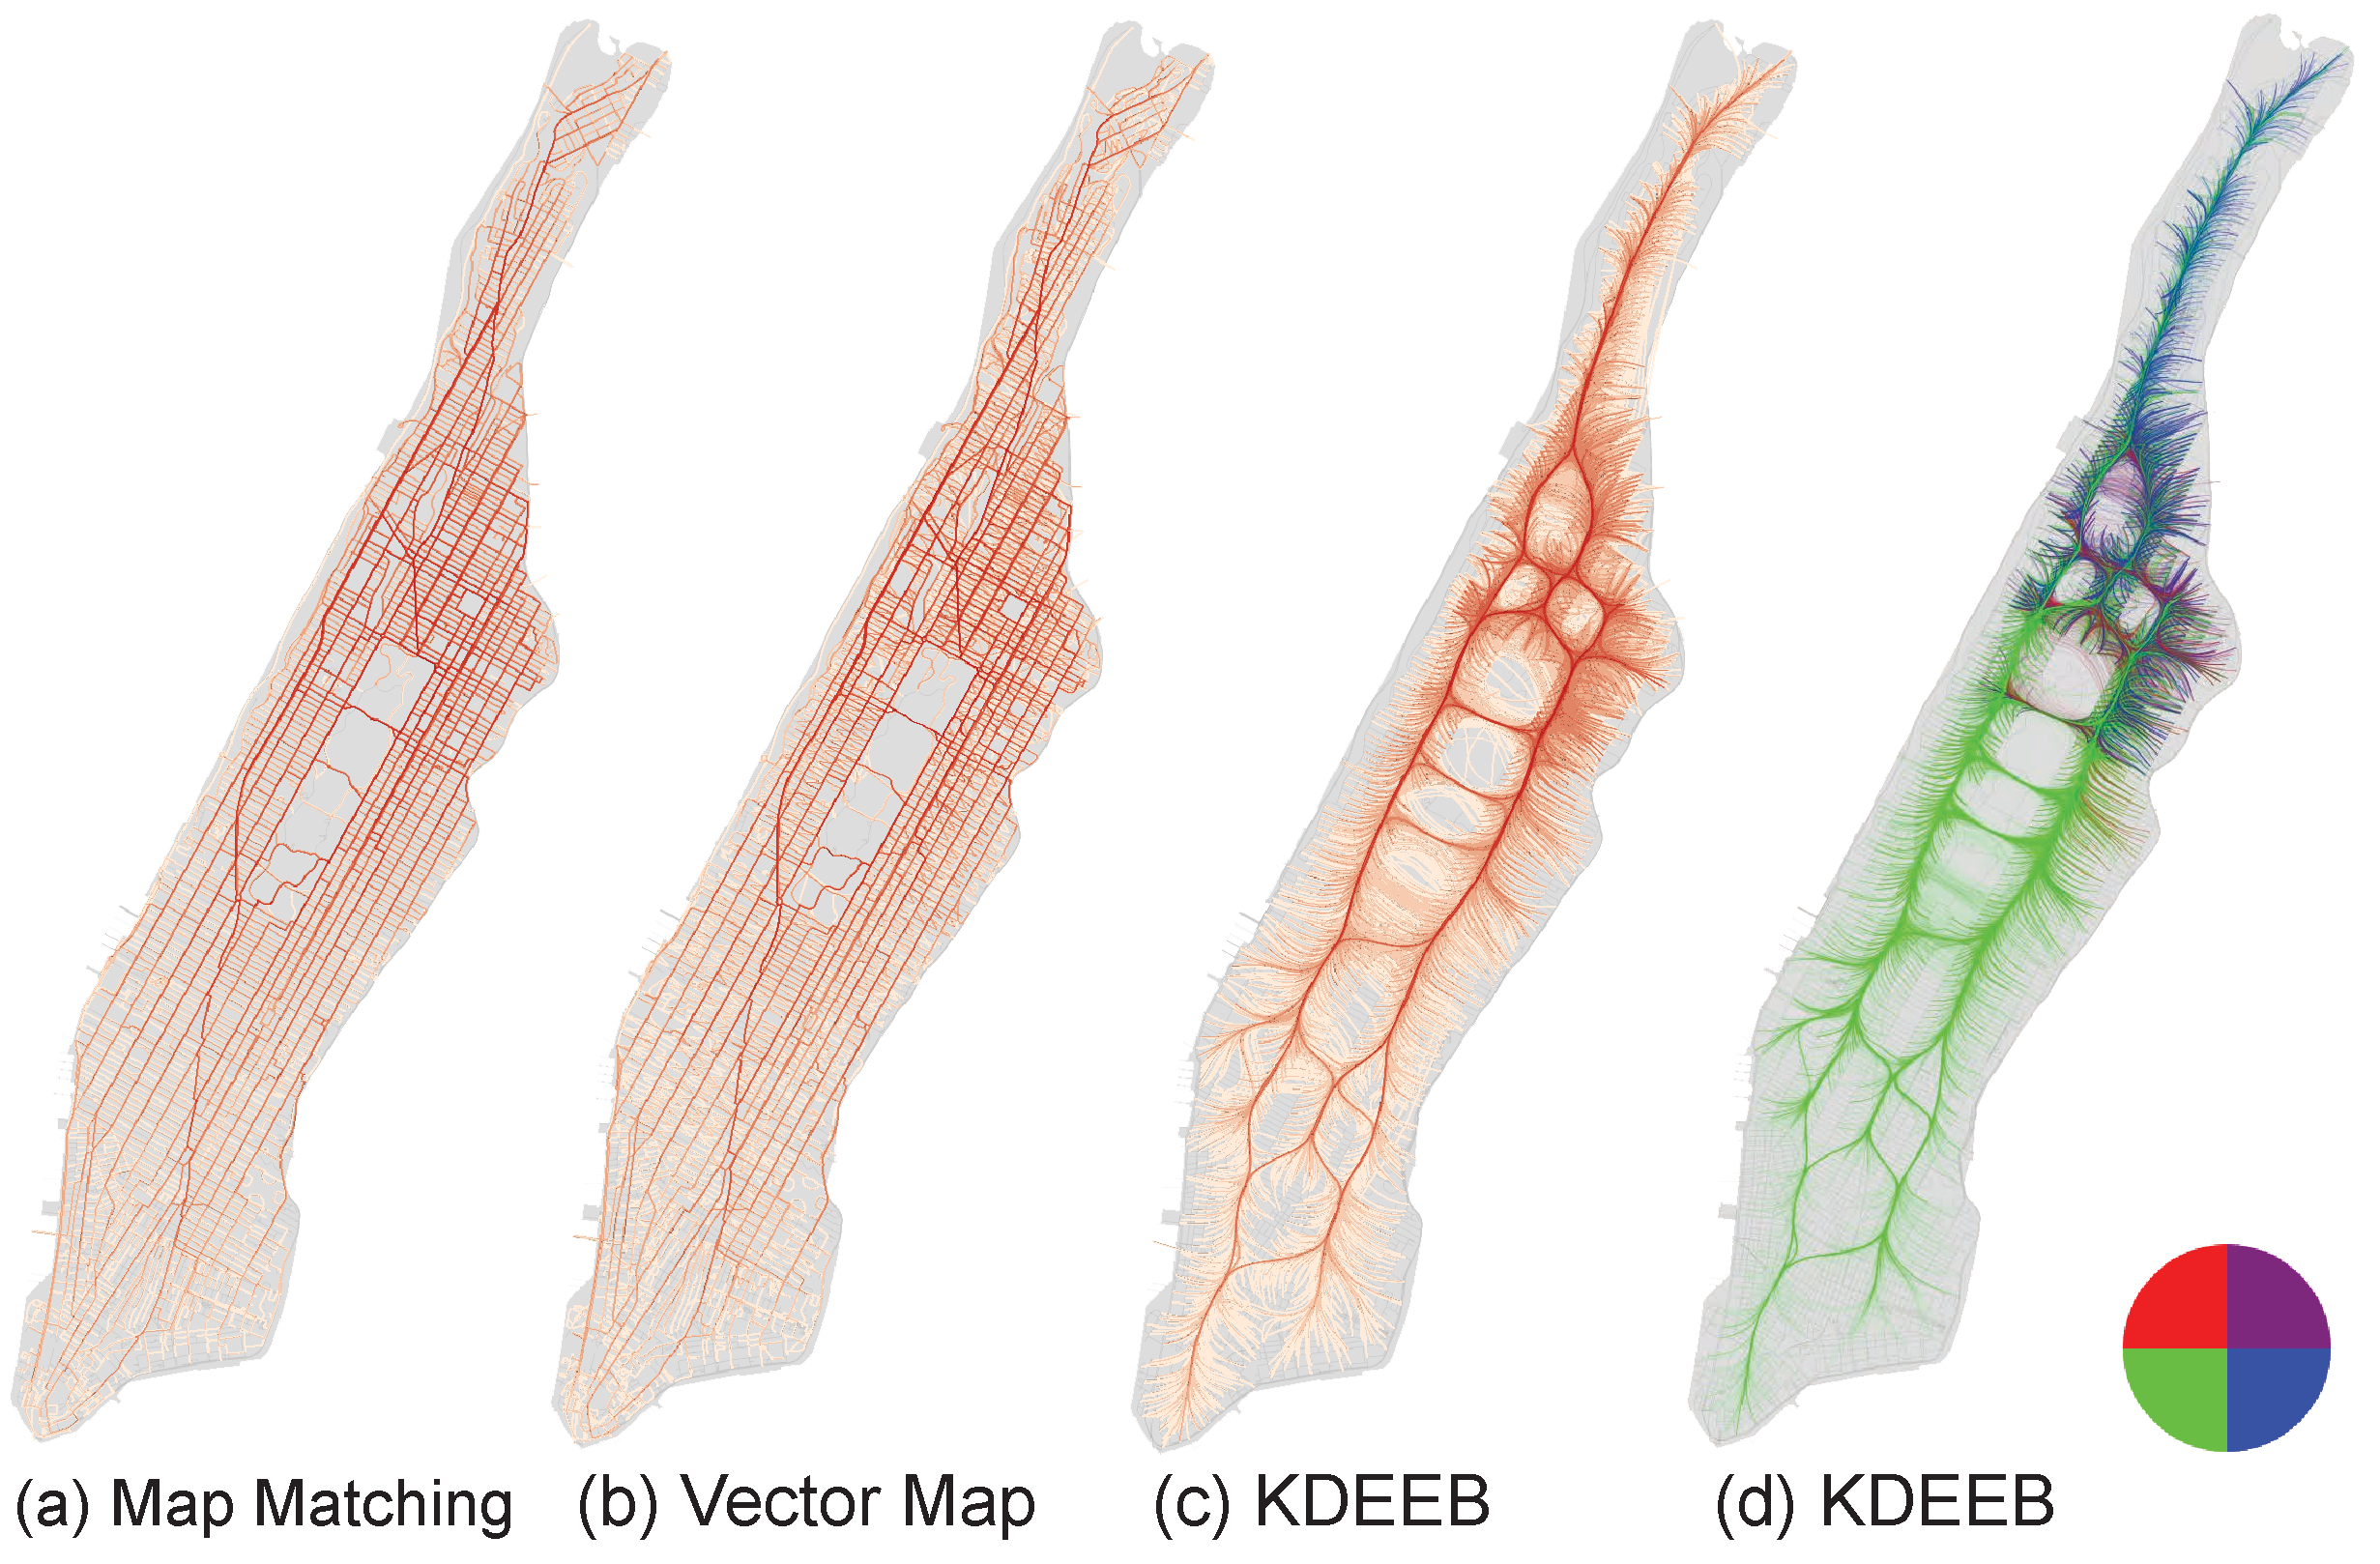
\includegraphics[width=0.495\textwidth]{fig1_alternatives/alternatives}
	\vspace{-6mm}
	\caption{Methods for visualizing OD trails in urban traffic: (a) map matching, (b) vector map, (c) \& (d) KDEEB bundles rendered in density and direction, respectively.}
	\label{fig:alternatives}
	\vspace{-5mm}
\end{figure}

%===================================================
\noindent
\textbf{Edge Bundling}.
To show individual OD trail, we treat ODs as nodes, and trails as links in a node-link graph, and employ edge bundling methods to reduce clutters.
Systematic overviews of state-of-the-art edge bundling techniques can be found in~\cite{zhou2013edge, lhuillier2017state}.
Here, we just give an overview.

Methods for general graphs can be categorized in three categories~\cite{zhou2013edge}.
\textit{Spring-based} methods model edges as springs, and generate bundled graph layout by assigning forces to the edges that can attract or repel each other (e.g.,~\cite{holten2009force}).
These methods usually suffer from high computational complexity and the processes are time-consuming.
\textit{Geometry-based} methods cluster edges based on potential control meshes in the input graph, which can be constructed through hierarchical graph drawing~\cite{holten2006hierarchical}, triangulation~\cite{zhou2008energy, lambert2010winding}, complex polygons~\cite{cui2008geometry}, and functional decomposition~\cite{hurter_2018_functional}.
Control meshes make geometry-based methods flexible and easy to control, yet the construction process can be time-consuming when the graph is large. 
\textit{Image-based} methods utilize image-processing to accelerate the bundling process.
Skeleton-based (SBEB~\cite{ersoy2011skeleton}) and kernel density estimation (KDEEB~\cite{hurter2012graph}) methods are developed in this category.
Compared with the other two groups of methods, image-based methods leverage GPU's powerful computing capacity, making them computationally efficient and scalable to handle millions of edges~\cite{van2016cubu, lhuillier2017ffteb}.

Besides, many edge bundling methods are developed targeting at improving certain features such as to minimize ambiguity~\cite{luo2012ambiguity, bach_2017_towards} and to reveal directional edge patterns~\cite{selassie_2011_divided}.
Some other methods are developed for specific applications such as to visualize geographical data in 3D~\cite{lambert20103d, thony2015vector} and neural connections in brain~\cite{2014_bottger_three-d, yang_2017_blockwise}.
Closely related to our work, vector map~\cite{thony2015vector} employs road network as a reference graph for edge bundling and represent the bundles as B-splines.
The approach is preferable for avoiding intersecting with obstacles in 3D, while marginal improvements are accomplished for urban traffic data on dense road networks.
Figure~\ref{fig:alternatives}(b) presents a vector map for Manhattan taxi trips in finest scale, which is very close to the original map as in Figure~\ref{fig:alternatives}(a).
In comparison, Figure~\ref{fig:alternatives}(c) \& (d) present KDEEB bundles with bundle lines colored in flow density and OD direction, respectively.
Main traffic roads and flow directions can be identified easily.
Nevertheless, there are many limitations of KDEEB when applied to urban traffic data.
We address these limitations with a new bundling method of RAEB.